% This file is the basic running of the model, just the population growth of Kiribati


\section{Demographics}
\subsection{Crude birth rate and death rate}
Births are modelled using time-variant crude birth rates that are multiplied by the modelled population 
size to determine the number of newborn individuals entering the youngest age category (0 - 4) at each time. A time-variant 
and age-specific rate of non-TB-related mortality applies to all model compartments to simulate 
deaths from other causes than TB. We use estimates from the UN Population Division\footnote{https://population.un.org/wpp/Download/Standard/Mortality/} to inform the 
birth and mortality rates.
We also apply additional death rates to the compartment I to reflect mortality induced by TB 
disease.
\begin{figure}[!ht]
    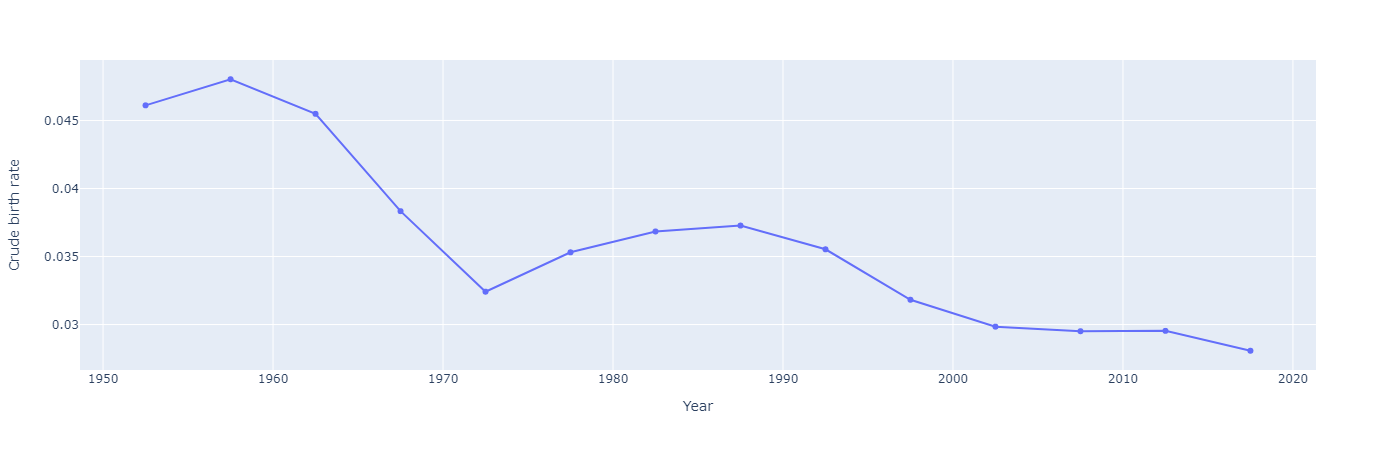
\includegraphics[width=\textwidth,height=\textheight,keepaspectratio,scale=0.6]{images/cbr.png}
    \caption{The crude birth rate of Kiribati from 1950 to 2020.}
    \label{fig:cbr}
\end{figure}

\begin{figure}[!ht]
    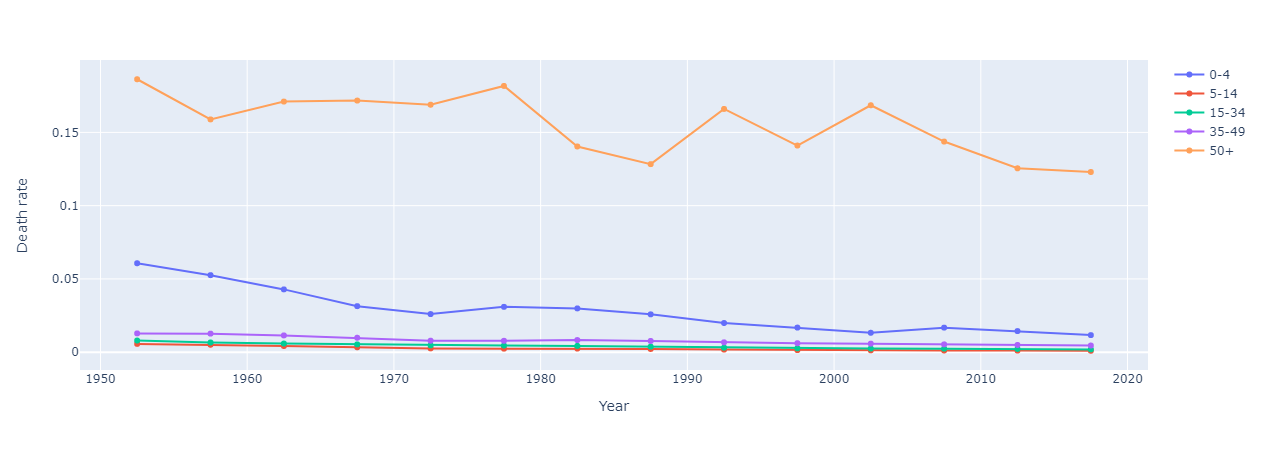
\includegraphics[width=\textwidth,height=\textheight,keepaspectratio]{images/cdr.png}
    \caption{The death rate of Kiribati from 1950 to 2020, stratified by age group.}
    \label{fig:cdr}
\end{figure}

\subsection{Comparing modeled population with actual population}
\begin{figure}[!ht]
    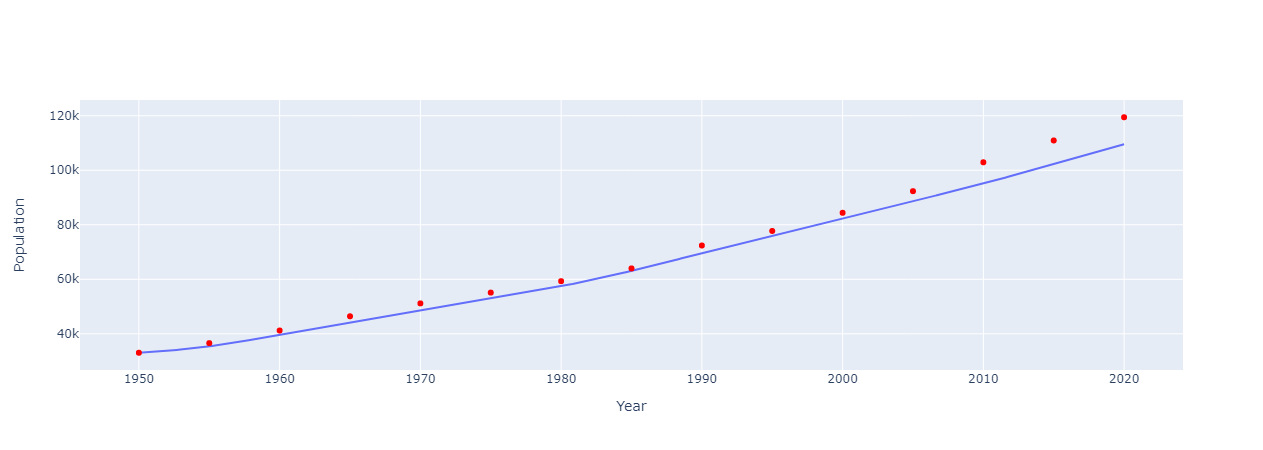
\includegraphics[width=\textwidth,height=\textheight,keepaspectratio]{images/modelled_total.png}
    \caption{Comparing modelled population with actual population of Kirbati from 1950 to 2020. The red dots represent the actual population size of Kiribati,
     while the blue line represents the modelled population size}
    \label{fig:modelled_total}
\end{figure}

\begin{figure}[!ht]
    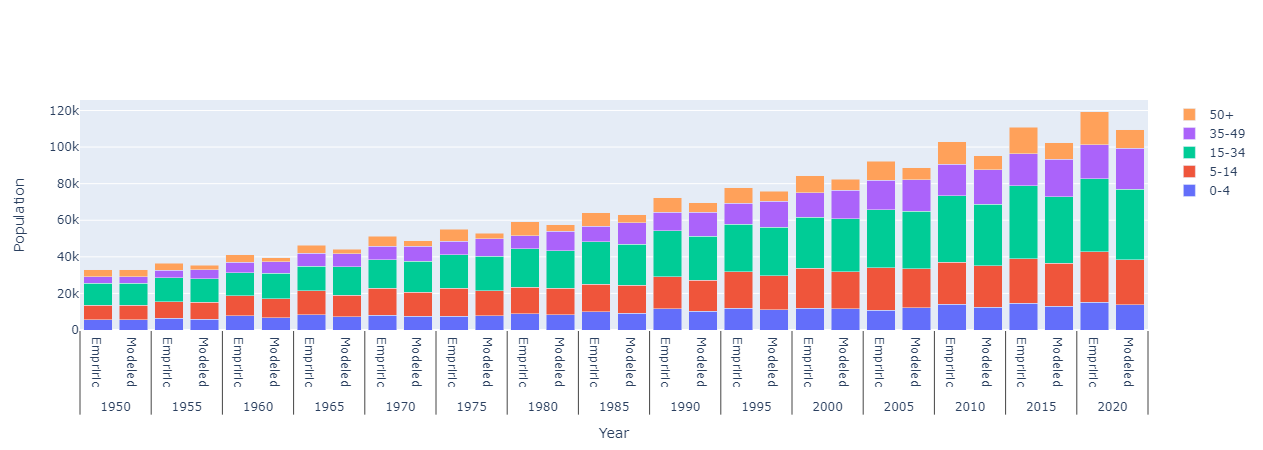
\includegraphics[width=\textwidth,height=\textheight,keepaspectratio]{images/compare_pop.png}
    \caption{Comparing modelled population with actual population by age groups of Kirbati from 1950 to 2020.}
    \label{fig:compare_group}
\end{figure}